%% software-and-experiments.tex  
% цей розділ висвітлює програмне рішенні та результати експериментів дослідження
\chapter{Об'єктно-орієнтоване програмне\ldots}\label{ch:03}

  Одним із найгнучкіших підходів до практичної реалізації нейромережевих технологій є створення програмного рішення. Цей підхід забезпечує можливість легкої модифікації реалізації порівняно з апаратними рішеннями\ldots 
  
\section{Структура та характеристики}
  
  При розробці програмного забезпечення було поставлено за мету використання виключно відкритого та вільного програмного забезпечення\ldots
  
  На рис.~\ref{fig:neurosimulator-modules} зображена компонентна діаграма розробленого програмного забезпечення із виділеними допоміжними модулями ресурсної взаємодії через Інтернет~\cite{Fie2000} та об'єктно-орієнтованої взаємодії з системами керування реляційними базами даних~\cite{ChGa2006}. 
  
  \begin{figure}[!htb]
    \centering
    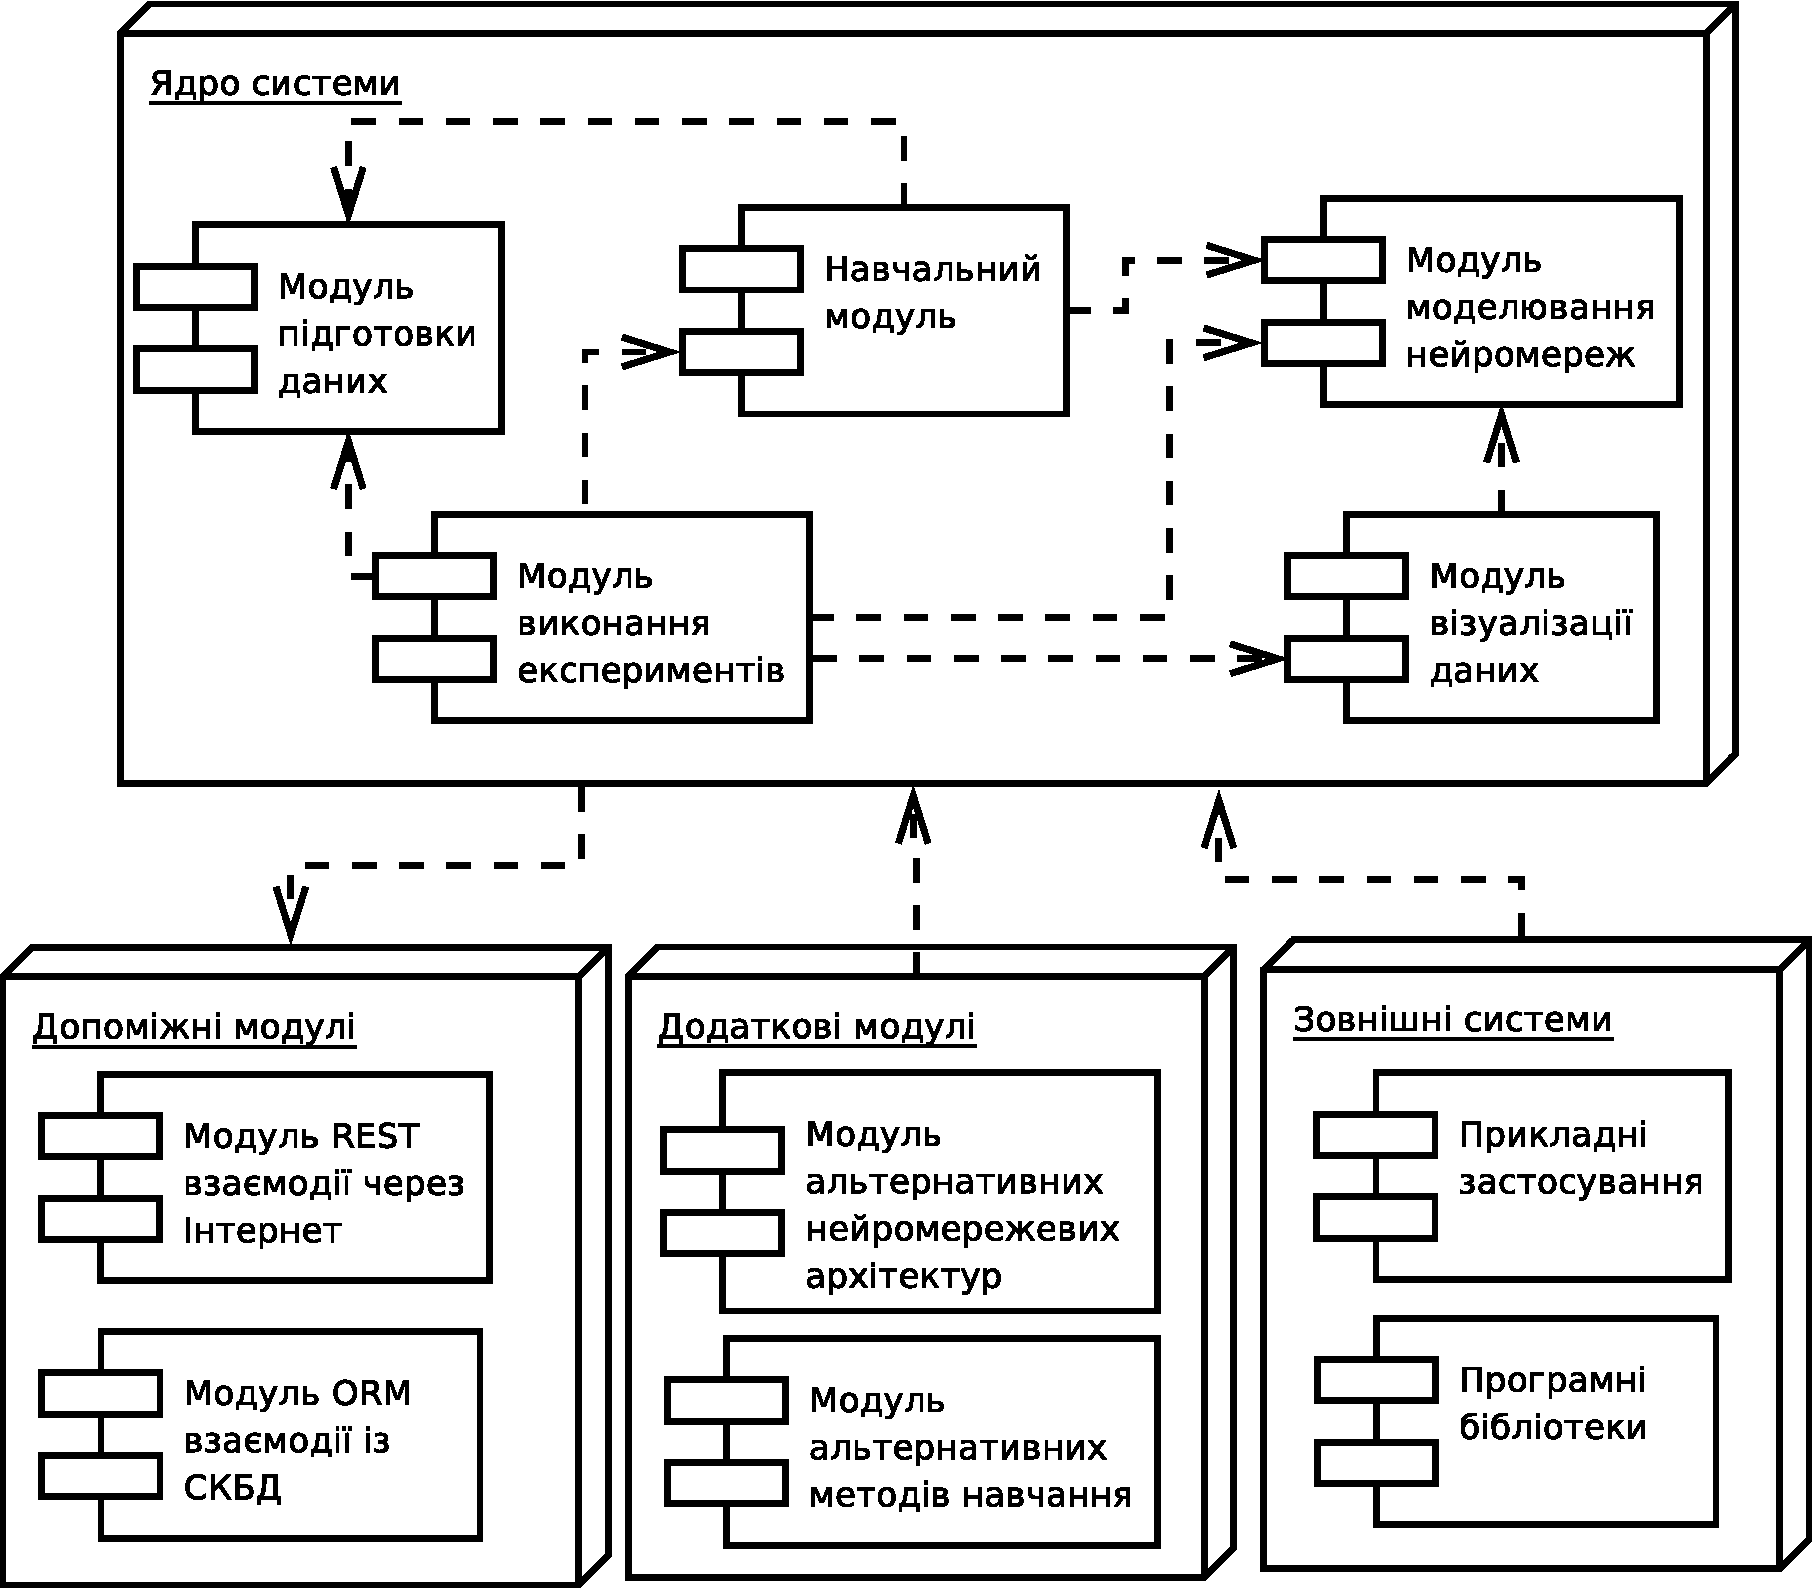
\includegraphics[scale=0.5]{chapters/03-software-and-experiments/images/01-neurosimulator-component-diagram.pdf}%
    \caption{Компонентна діаграма розробленого програмного забезпечення.}\label{fig:neurosimulator-modules}
  \end{figure}
  
  
\section{Обговорення коду}

\begin{lstlisting}
def filter(p: Tweet => Boolean): TweetSet
def filter0(p: Tweet => Boolean, 
            accu: TweetSet): TweetSet
\end{lstlisting}


\section{Висновки до розділу~\ref{ch:03}}